\documentclass[a4paper]{article}

\usepackage[utf8]{inputenc}
\usepackage[margin=1in]{geometry}
\usepackage[bookmarks]{hyperref}
\usepackage{graphicx}
\usepackage{listings}
\usepackage{color}
\usepackage{pdfpages}
\usepackage[style=verbose]{biblatex}
\usepackage{filecontents}
\usepackage{cleveref}
\usepackage[inline]{enumitem}
\graphicspath{ {images/} }

\def \IPF {\texttt{IPv4}}
\def \IPS {\texttt{IPv6}}

\author{Huw Jones\\27618153\\hcbj1g15@soton.ac.uk}
\title{COMP2207: Distributed Systems and Networks}
\def \subtitle {Distributed Notification Framework using Java RMI}


\hypersetup{
  pdfinfo={ee
    Title={\@title},
    Subtitle={\@subtitle}
    Author={\@author},
  },
  colorlinks=false,
  pdfborder=0 0 0,
}

\begin{filecontents}{bib.bib}
\end{filecontents}
\addbibresource{bib.bib}
\pagestyle{headings}

\begin{document}
\makeatletter
\begin{titlepage}
	\centering
	{\scshape\LARGE University of Southampton \par}
	\vspace{2cm}
    {\huge\bfseries \@title \par}
    \vspace{1cm}
	{\scshape\huge \subtitle \par}
	\vspace{3cm}
    {\Large
    \begin{tabular}{c}
      \@author
    \end{tabular} \\}
  \vspace{6cm}
    {\Large
    \today
    }
\end{titlepage}
\makeatother
\newpage

%%
%% SECTION: Notification Framework
%%
\section{Notification Framework}
As the notification system involved sinks, sources and notifications, it made sense to have 3 base classes: \texttt{NotificationSink}, \texttt{NotificationSource}, and \texttt{Notification}.
Java RMI requires interfaces to produce remote stubs, so, I extracted the publicly accessible remote methods into the respective interfaces (\texttt{INotificationSource} and \texttt{INotificationSink}).
Also, I made sure that both \texttt{NotificationSink}, \texttt{NotificationSource} extend \texttt{UnicastRemoteObject} to allow the dynamic creation of the remote method stubs.
This means that Sinks/Sources can be used directly in remote methods.

\subsection{Interfaces}
The coursework set out a subscribe-publish system, therefore I decided that the following methods must be present in the interfaces for the framework to properly function.
In \texttt{INotificationSource}:
\begin{enumerate}
  \item \texttt{UUID} \texttt{register(INotificationSink)} - Registers a sink and returns the assigned UUID of the sink
  \item \texttt{boolean} \texttt{register(UUID, INotificationSink)} - Registers a sink with the UUID, returns if the sink was registered or not
  \item \texttt{boolean} \texttt{isRegistered(INotificationSink)} - Returns if the sink is registered
  \item \texttt{boolean} \texttt{unregister(UUID)} - Unregisters the sink by UUID and returns if the sink was unregistered
  \item \texttt{boolean} \texttt{unregister(INotificationSink)} - Unregisters the sink and returns if the sink was unregistered
\end{enumerate}
and in \textbf{INotificationSink}:
\begin{enumerate}
  \item \texttt{void} \texttt{notify(Notification)} - Notifies the Sink of a new Notification.
\end{enumerate}

The base classes, \texttt{NotificationSink} and \texttt{NotificationSource}, implemented useful methods that I believed all sinks/sources required.
Both classes had a \texttt{ShutdownHandler} thread that was hooked to the JVM shutdown and made sure the sink/source shutdown gracefully.


\subsection{Notification}
My \texttt{Notification} class has these properties: SourceID, Time, Priority and Data.
\texttt{Notification} is a generic that allows the data to be any  subclass of \texttt{Serializable}.
This ensures that applications that use the framework will not compile if objects that are \textbf{not} serialisable are sent in a Notification.
The SourceID field allows sinks to use callback functions to handle notifications from different sources, and Time is a timestamp from when the source sent the notification.
Although \texttt{Notification} features a priority field, the framework does not use this.

\subsection{Notification Source}
\texttt{NotificationSource} implements common features that all Sources need.
Such features include sink registry management, RMI registry binding, sending notifications, and session resumption.
\texttt{NotificationSource} provides standardised registry binding methods to bind to any server on any port.
It also provides a single method to send (publish) notifications to all sinks using the sink registry management.
In addition, the code to handle lost connections is also tied in here.
This allows an application's source to call\texttt{sendNotification(Notification)} to publish a notification and the framework handles the message and delivery.

\texttt{NotificationSource} features a thread worker pool that is used to send notifications.
Each thread in the pool sends a notification to one source.
This feature was added to mitigate lost connections, but had the side effect of allowing the source to more efficiently handle multiple sinks.
See \Cref{sec:lost_conns} for more details.

\subsection{Notification Sink}
\texttt{NotificationSink} has methods to abstract gracefully connecting/disconnecting from sources and handling notifications.
When a sink registers with a source, the framework provides the ability for a callback function to be executed for that source.
This allows the Sink to be able to handle the notifications from different sources effectively.
For example, a Sink connected to a CCTV system Source would either want to display the image, or save it.
But, a Sink registered to a text based weather Source would not be able to display this data as an image.
The framework allows one sink to register to multiple sources and attach a different handler to each source;
e.g.: display the CCTV image, parse the weather data and display it on matrix display.

%%
%% SECTION: The Application
%%
\section{Application}
For the application, I decided to simulate a CCTV system using GIFs.
Each camera is a Source, and each client is a sink.
A CCTV system requires clients to be able to connect to all the cameras, and multiple clients to connect to the same camera.
This application model directly matches that of the framework and it is the perfect candidate to test the framework.
I am modelling cameras using animated GIFs because I deemed it too complicated to set up cameras/webcam.
My Java source zip contains a selection of cat gifs and config files. The application has 2 main classes:
\begin{enumerate*}
  \item Client
  \item GifStreamer
\end{enumerate*}.
The diagram in \Cref{sec:system_diagram} shows how the application uses the framework and shows the class inheritance.

\subsection{Client}
The \texttt{GifClient} provides a GUI to connect to an RMI server and bound sources.
The \texttt{GifClient} has a \texttt{NotificationSink} that is used to connect to sources.
When the sink registers, it opens a new window to view that source.
If a window is closed, the client uses framework code to unregister from the source.
The client features a combobox to select the source if the optional framework component \texttt{SourceProxy} is running (see \Cref{sec:source_proxy}), otherwise the user can type the Source ID into a text box.

It also features a config file system that allows the Client UUID to be stored, as well as automatically connecting to sources when the application runs.
The autoconnect feature would be useful for systems where you would like the client to autoconnect to the cameras.

\subsection{Source}
The \texttt{GifStream} class extends \texttt{NotificationSource}.
It loads a GIF file, extracts each frame and converts it to a byte array (\texttt{BufferedImages} are not serialisable).
When it has converted the GIF, it tries to register with the \texttt{SourceProxy}, or binds directly to the RMI registry (if localhost), otherwise it fails to start up.
The GIF file is specified by a config file.
When starting the source, config files are specified by using a \texttt{-c [PATH]} flag, or if the flag is not specified, the config loader tries to load \texttt{server.conf}.
Config files specify the RMI server to connect to (if not localhost:1099) as well as the SourceID (that the client sees).
There is a \texttt{source} declaration that specifies the path to the GIF file source.

\subsection{Testing}
To test the framework, I started the rmiregistry on my computer.
I found some gifs, created config files and started the sources.
I ran the client on my laptop and connected over Wifi to the sources.
The, I began to test all the different scenarios: connecting, disconnecting, network issues, etc.

This became tedious, so I created some helper scripts to start the applications for me.
These scripts are included in the source zip.

To run the application, first make sure the application has been built (run \texttt{build.sh} or \texttt{build.bat}).
Then navigate to the \texttt{run} directory.
To run the client, run either \texttt{./Client.sh} or \texttt{Client.bat}.
To run sources, run either \texttt{./GifSource.sh -c [path to config file]}, or \texttt{GifSource -c [path to config file]} - this will start a source using a specified config file.
There are 4 provided config files and gifs in the source zip.
In order to connect to a source, type the source ID into the client and click connect - the source ID for the source is printed to the source console when it starts up.
Please note the \texttt{rmiregistry} is automatically started when running \texttt{GifSource.sh}, \texttt{GifSource.bat}, \texttt{SourceProxy.sh}, \texttt{SourceProxy.bat}.

To use the optional \texttt{SourceProxy} middleware, make sure \texttt{SourceProxy} is started before the sources/sinks.

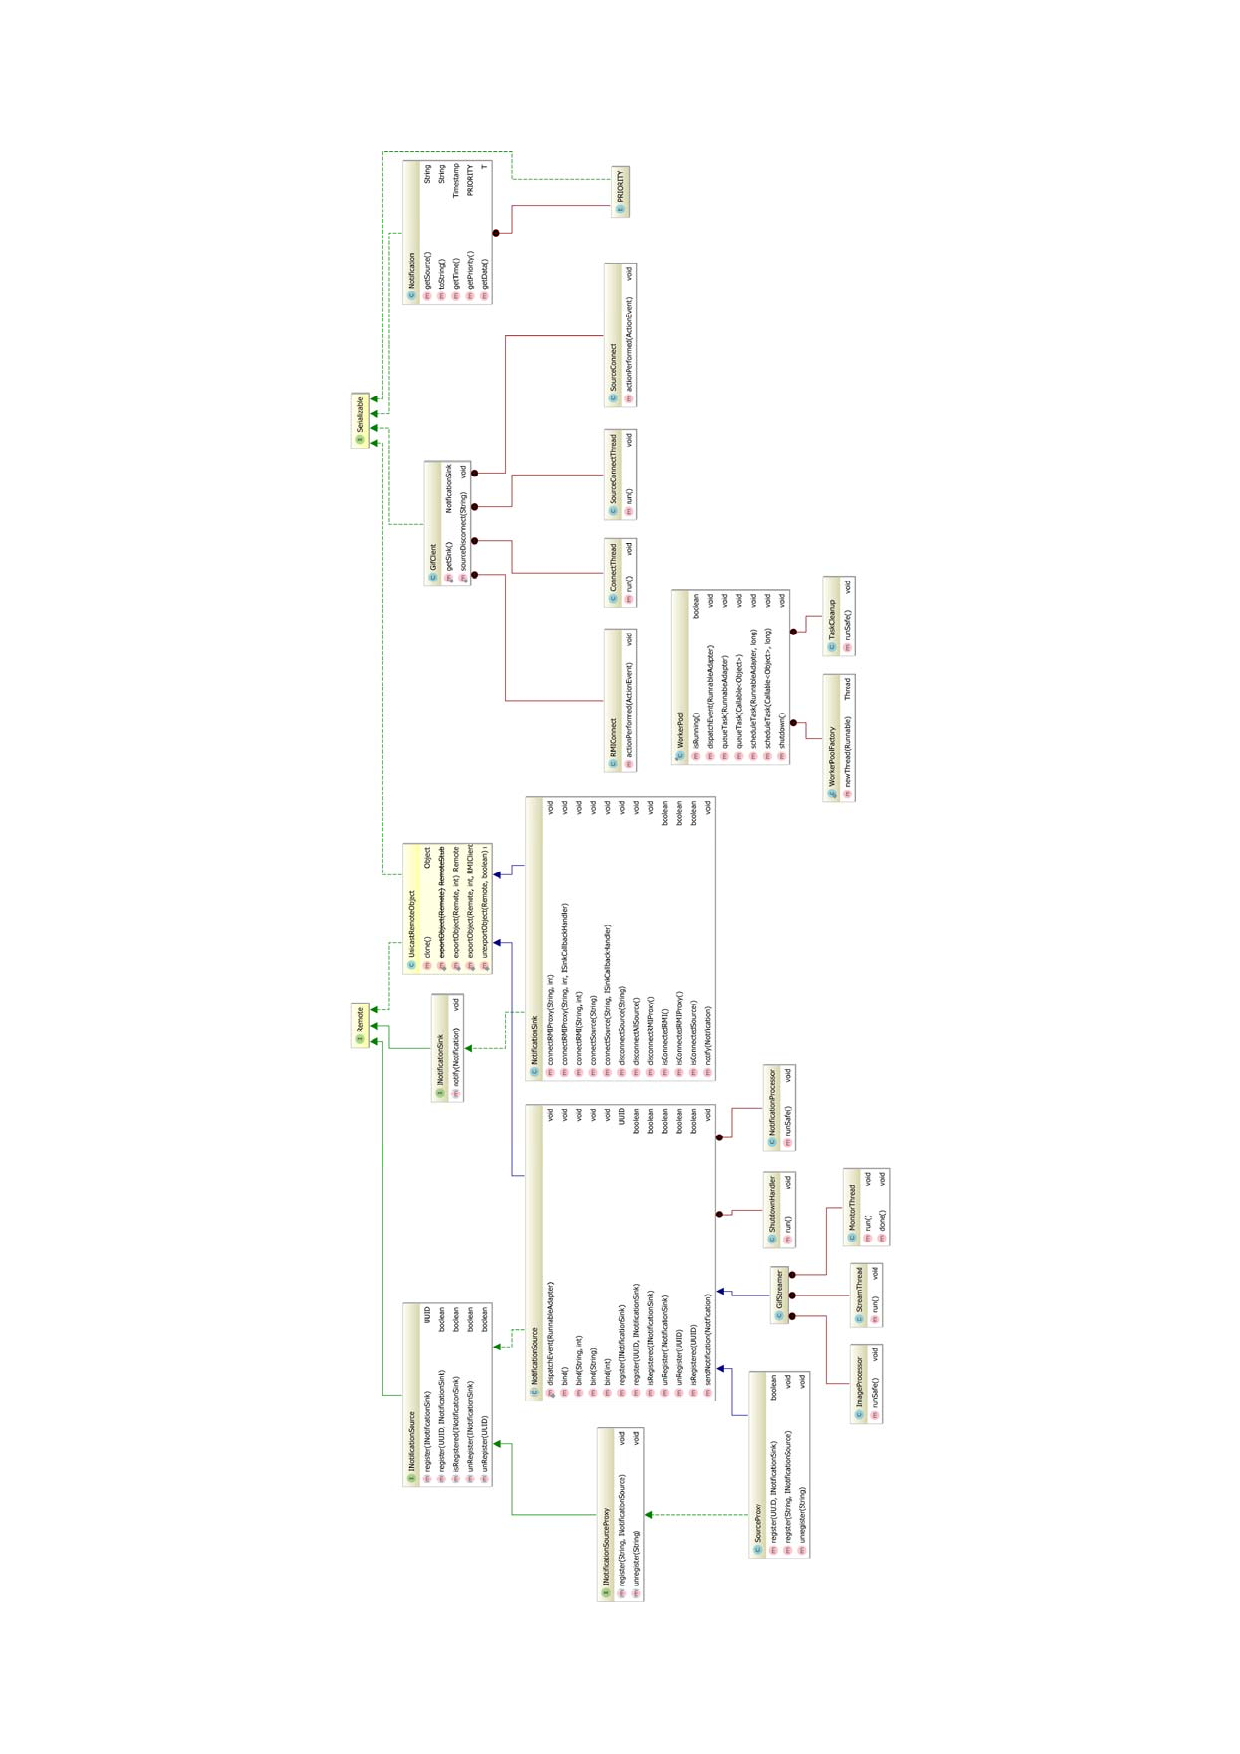
\includepdf[landscape=false,scale=0.9,pagecommand={\subsection{System Diagram}\label{sec:system_diagram}}]{SystemDiagram.pdf}

%%
%% SECTION: Sources and Sinks
%%
\section{Sources \& Sinks}
To test multiple sinks and sources, I ran 3 sources and 3 sinks.
\Cref{fig:testing} is a screenshot whilst testing my application.
The consoles for the 3 sources are on the left side and both clients are on the right side.
There are 4 windows open: 2 for each client, 1 for each source.
This screenshot proves that multiple sinks can register with multiple sources and one sink can register with multiple sources.
The 3rd sink was running on my computer and was receiving notifications.

\begin{figure}[h]
\includegraphics[width=\textwidth]{testing}
\caption{Screenshot of testing.\label{fig:testing}}
\end{figure}

%%
%% SECTION: Lost Connections
%%
\section{Lost Connection}\label{sec:lost_conns}
RMI is connectionless as there is no constant link between 2 remote objects.
This means that after calling a remote method, there is no way to know if the remote object is still available next method call.
The only way to tell is to call the method and wait for the Socket to timeout and a \texttt{RemoteException} to be thrown.

\subsection{Resending Notifications}
Lost connections are handled by the framework and the application is oblivious that a notification failed to send - the framework guarantees that it will deliver the notification\textellipsis eventually.

To handle ``lost connections'', \texttt{NotificationSource} catches the \texttt{RemoteException} and queues the notification against the sink's UUID to resend later.
Even though notification sending failed, the source still attempts to send further notifications.
This means that when the source is able to send notifications, or the sink reregisters (registers with the same UUID and updates its remote reference),
the method \texttt{NotificationSource::sendQueue(UUID sinkID)} is called.
This method attempts to send all notifications in the queue for the sink.
If any notifications fail to send, it stops trying to send the rest of the queue and tries again when the next notification is sent successfully.

This method to handle lost connections requires a large amount of free memory to store all the unsent notifications;
 if a sink disconnects without unregistering, or fails to reregister, the source will store all the missed notifications.
Eventually the JVM will run out of memory.
To solve this, the oldest notifications could be removed when the source starts to run out of free memory (e.g.: 10\% free space).

\subsubsection{Unintended Consequences}
Due to the application high throughput (notifications are sent on average 15 times a second), it was very noticeable when a sink disconnected or notifications failed to send.
Given 2 sinks both connected to the same source and a sink drops connection.
The initial framework was single threaded, so when the source failed to send notifications to the sink, the source froze whilst sending messages.
This was caused by a high socket timeout and the framework send notifications serially on the same thread.

To prevent a lost connection from affecting a Source's ability to continue to notify ``alive'' sinks, I added a Thread Pool to the \texttt{NotificationSource} class.
The framework now sends notifications on a thread in the Thread Pool instead of running it on the Source thread.
With a big enough thread pool, this means as long as not all the threads are blocked whilst waiting for the RMI socket to time out, the Source can still send notifications to sinks.
In addition, I created an \texttt{RMISocketFactory} to reduce the socket timeout and consequently, the maximum time the send threads were blocked for.

%%
%% SECTION: Future Work
%%
\section{Future Work}
\subsection{Source Proxy}\label{sec:source_proxy}
The application can already be run over different machines using \texttt{SourceProxy}.

Java applications cannot bind remote objects on foreign (non-localhost) RMI registry server.
As a workaround, I created a proxy class to bind the sources.

With \texttt{SourceProxy} running, the application flow is:
\\begin{\begin{enumerate}
  \item Start \texttt{remiregistry} on Server1.
  \item Start \texttt{SourceProxy} on Server1.
  \item Start any \textbf{Source} on any server with a config file that uses Server1. (E.g.: \texttt{server: Server1,1099;})
  \item Source registers with \texttt{SourceProxy} on Server1 and \texttt{SourceProxy} binds the remote object to Server1's RMI registry.
  \item Start any client on any computer.
  \item Connect client to Server1.
  \item Client registers with \texttt{SourceProxy}.
  \item \texttt{SourceProxy} sends a list of registered sources to client (and continues to notify Client of Source changes).
  \item Client looks up source (from list from Proxy) on registry server.
  \item Client connects to source on source's server.
\end{enumerate}}

\subsection{Improvements}
After implementing multithreading in the framework to send notifications, there have been some cases where notifications ``fail to send''.
This is probably due to the notification being sent in a different thread.
I don't believe the bug prevents all the queued notifications from being sent, but it writes a lot of errors to the source's console.

%%
%% SECTION: Conclusions
%%
\section{Conclusions}
Overall, I do not believe Java RMI is suitable for any distributed object system.
It is too buggy and fiddly to get it to work easily and reliably across multiple hosts.
Information on how to use RMI is not centrally located, and when it is, some of it is out of date or fails to mention important issues.
The Oracle website has a plethora of RMI guide and tutorials targeting different versions of Java, not located together.
Even for tutorials targeting the same version of Java, two different tutorials/guides contradict on how RMI works.

That said, when you find all this information and spend hours gleaning over the internet (see https://xkcd.com/979/),
RMI works really well.
However, I strongly dislike the fact that RMI ``hides'' things - I prefer raw Socket based communication, or using stream wrappers on sockets.

For a publish-subscribe notification system, I don't believe RMI is the best solution.
I would choose sockets every time given the choice  of sockets or RMI.
If I had to choose how I implemented the notification system, I would have had Sources broadcasting UDP packets saying they are sending notifications of x type on y ip on z port.
The client would listen for these packets and create a list to present to the end user.
The end user connects via a TCP socket that is kept alive using a heartbeat or blocking thread, and the source sends notifications over this socket.
Yes, this would require a lot more work to build a framework, but after having already built a similar framework for COMP1206 Auction System,
I still feel the amount of work is justified to not have to use Java RMI.

\end{document}
